\documentclass[conference]{IEEEtran}
\IEEEoverridecommandlockouts
\usepackage[T1]{fontenc}
% The preceding line is only needed to identify funding in the first footnote. If that is unneeded, please comment it out.
\usepackage{cite}
\usepackage{amsmath,amssymb,amsfonts}
\usepackage{float}
\usepackage[hidelinks]{hyperref}
\usepackage{booktabs}
\usepackage{multirow}
% \usepackage{subcaption}

\usepackage{graphicx}
\usepackage{textcomp}
\usepackage[normalem]{ulem}
\usepackage{xcolor}
\newcommand{\AD}[1]{}
\newcommand{\Long}[1]{}
\def\BibTeX{{\rm B\kern-.05em{\sc i\kern-.025em b}\kern-.08em
    T\kern-.1667em\lower.7ex\hbox{E}\kern-.125emX}}

\DeclareMathOperator*{\argmin}{arg\,min}

\makeatletter
\newcommand{\linebreakand}{%
  \end{@IEEEauthorhalign}%
  \hfill\mbox{}\par
  \mbox{}\hfill\begin{@IEEEauthorhalign}%
}
\makeatother


\DeclareMathOperator{\diag}{diag}

\begin{document}

\title{Communication-Efficient ADMM Using Multitask Gaussian Processes
\thanks{This material is based upon work supported by the National Science Foundation under Awards No. 2449927 and 231711.}
}

% \author{\IEEEauthorblockN{Long Vu}
% \IEEEauthorblockA{\textit{Electrical and Computer Engineering} \\
% \textit{Louisiana State University}\\
% Baton Rouge, LA \\
% dvu29@lsu.edu}
% \and
% \IEEEauthorblockN{Aldo Duarte}
% \IEEEauthorblockA{\textit{Electrical and Computer Engineering} \\
% \textit{Louisiana State University}\\
% Baton Rouge, LA \\
% aduart3@lsu.edu}
% \linebreakand
% \IEEEauthorblockN{Truong X. Nghiem}
% \IEEEauthorblockA{\textit{Electrical and Computer Engineering} \\
% \textit{University of Central Florida}\\
% Orlando, FL \\
% truong.nghiem@ucf.edu}
% \and
% \IEEEauthorblockN{Shuangqing Wei}
% \IEEEauthorblockA{\textit{Electrical and Computer Engineering} \\
% \textit{Louisiana State University}\\
% Baton Rouge, LA \\
% swei@lsu.edu}}

\author{
\IEEEauthorblockN{
Long Vu\IEEEauthorrefmark{1},
Aldo Duarte\IEEEauthorrefmark{1},
Truong X. Nghiem\IEEEauthorrefmark{2},
and Shuangqing Wei\IEEEauthorrefmark{1}
}
\IEEEauthorblockA{
\IEEEauthorrefmark{1}Electrical and Computer Engineering,
Louisiana State University, Baton Rouge, LA, USA\\
Email: \{dvu29, aduart3, swei\}@lsu.edu
}
\IEEEauthorblockA{
\IEEEauthorrefmark{2}Electrical and Computer Engineering,
University of Central Florida, Orlando, FL, USA\\
Email: truong.nghiem@ucf.edu
}
}

\maketitle

\begin{abstract}
The Alternating Direction Method of Multipliers (ADMM) is a well-known method for solving convex distributed optimization; however, it requires frequent query-response exchanges between the coordinator and distributed agents until convergence. In environments where communication between the coordinator and agents is costly, reducing unnecessary queries while preserving the algorithm's performance is crucial. 
In this work, we propose a Multitask Gaussian Processes (MTGP) approach to reduce the number of exact queries required to solve a distributed convex sharing problem.  
Using the relationship between the Moreau envelope and the proximal operator, a derivative-aware MTGP jointly learns agents' Moreau envelopes and their gradients, allowing observations from one agent to inform predictions of other agents' proximal updates. 
Furthermore, we investigate how agent structure affects the proposed method's performance by intentionally constructing cluster-wise function datasets in which each agent's objective function within a cluster is similar. We consider a global model that shares information across all agents and a cluster-wise variant that uses known agent-group labels. We also provide an adaptive querying method based on prediction uncertainty, and we refine the prediction result using gradient projection onto a feasible set constructed by past queries. We evaluate our proposed algorithm on a distributed quadratic programming problem under various cluster structures and scenarios. The empirical results show that MTGP reduces exact agent queries by $76.25$--$80.77\%$ with relative objective discrepancy below $0.01\%$ from the exact-update ADMM baseline and $1.03$--$1.28$ times its iteration count. These results use instance-specific tuning on six synthetic quadratic instances. Known group labels yield small, mixed changes in query cost.

% Additionally, the results also show that knowing the cluster structure of local functions yields stable reductions in exact queries and fewer query-active iterations, as well as lower computational cost in modeling MTGP.
\end{abstract}

\begin{IEEEkeywords}
Distributed Optimization, ADMM, Gaussian Processes, Multitask Gaussian Processes
\end{IEEEkeywords}

\section{Introduction}

Distributed optimization enables multiple agents to solve a coupled optimization problem through local computations and information exchange. In coordinator-based sharing problems, each agent contributes a local objective, while a shared cost couples the agents' decisions. 
The alternating direction method of multipliers (ADMM) is a well-known algorithm for distributed optimization that solves such problems \cite{boyd2011distributed}. 
This algorithm splits the main problem into smaller subproblems that each subsystem can solve and update in a \textit{Gauss-Seidel} style. 
In this scheme, each agent's local subproblem is cast as a \textit{proximal minimization problem} \cite{10.1561/2400000003}, which adds a scaled quadratic regularization term to the objective. During execution, the agents send the solution of their local subproblem to the coordinator, which aggregates the solution information and broadcasts new queries that steer the local objectives toward the global objective.
% \AD{This sentence as a whole is weird to read, there are plural/singular inconsistencies and the idea of what you want to say is confusing}. 
This algorithm is simple, yet easy to implement, and well-suited to parallel computation; hence, many applications in other fields have been developed recently, as in \cite{er2024distributed, 10443910, 11143820, he_admm_2025}. 

However, distributed optimization algorithms and ADMM often require many iterations to converge, which in turn require repeated query-response exchanges between agents and the coordinator. As a consequence, in systems where communication is particularly time-consuming due to delays, loss, or energy limitations (e.g., batteries or solar power), as in remote wireless sensor networks, developing reliable communication can be costly. Therefore, reducing these exchanges while retaining solution accuracy is an important objective. Extensive work has aimed to improve communication efficiency in distributed optimization without significantly sacrificing the original algorithm's performance, as in \cite{JMLR:v18:16-512, pmlr-v108-li20f, duarte2024communication, 8673589}.

% This is particularly relevant when transmission consumes limited energy, bandwidth, or time \AD{This is not necessarily true for transmission being costly; yesterday you wrote this part more clearly}.

A complementary approach that enables the coordinator to estimate agent proximal updates and skip unnecessary queries when the estimate is sufficiently reliable was first proposed in \cite{stathopoulos2018communicationreductiondistributedoptimization}.  This approach uses the relationship between the proximal operator and the gradient of the Moreau envelope. 
This envelope provides a differentiable scalar function whose gradient can be used to calculate the solution of the proximal minimization problem, making it a suitable target for learning from previous query responses. 
Motivated by this idea, the authors in \cite{8635898, duarte2024optimal} proposed \textit{STEP-GP}, which uses Gaussian Processes (GP) to approximate the Moreau Envelope and its gradient, while also proposing multiple adaptive-query schemes to reduce communication overhead. A recent development of this approach, \cite{duarte2026communication}, proposed adaptive quantization to further reduce communication overhead when solving the distributed sharing optimization problem using ADMM. 
Although these methods show substantial communication efficiency, there are open avenues to further reduce communication costs and explore the structure and dynamics of queries between agents and the coordinator. In this work, we aim to answer two research questions (RQ):

\begin{enumerate}
     \item \textbf{RQ1}: In STEP-GP, each agent's Moreau Envelope is modeled individually with GPs to predict new query points. However, when the functions are highly correlated, can we leverage this correlation to improve prediction results and reduce the number of additional exact query rounds required?
     \item \textbf{RQ2}: When the set of $N$ agents can be grouped cluster-wise, and functions in the same cluster are considered highly correlated. Does the information about the structure or label of each function provide additional benefit when using a surrogate model to estimate the Moreau Envelope and its gradient?
\end{enumerate}

In this paper, we address these questions by leveraging correlations between agents' local functions. We develop a Multitask Gaussian process (MTGP) model with an adaptive query method to jointly learn the Moreau Envelope function to leverage potential shared information between agents. In addition, we structurally generate cluster-wise local functions to study the effect of inter-cluster structure and agents' query behavior when using a GP-based surrogate model. The main contributions of our work are as follows:

\begin{itemize}
    \item We leverage the structural relationship between the Moreau Envelope and the Proximal Operator to develop an MTGP model with an adaptive decision-query mechanism that improves ADMM communication efficiency while maintaining algorithmic effectiveness.

    \item We investigate the effect of function similarity and the clustered structure of agents' objective functions on modeling the MTGP to reduce exact queries when solving the distributed optimization problem
    
    \item We validate the effectiveness of the proposed method across various of cluster structures. The results show that our approach significantly reduces the number of exact agent queries required by the ADMM algorithm while maintaining high accuracy.
\end{itemize}

The remainder of this paper is organized as follows. We first define the distributed sharing problem and the subtle connection between the Moreau Envelope and the proximal operator in Section~\ref{sec:problem_formulation}. Then, in Section~\ref{sec:mtgp_with_derivative}, we describe the MTPG method 
%of Multitask Gaussian Process 
with derivative information for jointly learning the proximal operator with an adaptive query method. 
Section~\ref{sec:data_generate} defines the datasets and evaluation protocol, and Section~\ref{sec:simulation_result} presents the results and discussion. The paper concludes with future research directions in Section~\ref{sec:conclusion}

\section{Distributed Sharing Optimization and Proximal Operator Estimator}
\label{sec:problem_formulation}

\subsection{Problem Formulation}

Consider a distributed sharing optimization algorithm with \textit{N} agents and a central coordinator with the form:
\begin{align}
    \text{minimize} \sum_{i=1}^{N} f_i (x_i) + g(\sum_{i=1}^N x_i)\text,
    \label{distributed_shairing}
\end{align}
where $x_i \in \mathbb{R}^p$ and $f_i: \mathbb{R}^p \mapsto \mathbb{R}, \ i = 1, \dots, N$ are local convex functions that are private and correspond to each agent. The shared global cost function $g: \mathbb{R}^p \mapsto \mathbb{R}$ is also a proper convex function. 
This problem can be written in ADMM form by introducing the copies $z_i$ of $x_i$ as follows:
\begin{equation}
    \begin{aligned}
    \text{minimize} \sum_{i=1}^{N} f_i (x_i) + g(\sum_{i=1}^N z_i)\text, \\
    \text{s.t:} \quad x_i - z_i = 0, \quad i = 1, \dots, N
\end{aligned}
\end{equation}
with $z_i \in \mathbb{R}^p$. %, i = 1, \dots, N$. 
For solving (\ref{distributed_shairing}), the ADMM algorithm iteration can be viewed as:
\begin{equation}
\begin{aligned}
    x_i^{k+1} &= \argmin_{x_i \in \mathbb{R}^p} \left \{ f_i(x_i) + \frac{\rho}{2}\|x_i - y_i^k\|_2^2) \right \} \\
    \bar z^{k+1} &=  \argmin_{\bar z \in \mathbb{R}^p} \left \{ g(N \bar z) + \frac{N\rho}{2}\|\bar z - u^k - \bar x^{k+1}\|_2^2 \right \} \\
    u^{k+1} &=u^k + \bar x^{k+1} - \bar z^{k+1}\text,
\end{aligned}
\label{eq:admm_sharing_algorithm}
\end{equation}
% where $y_i^k = x_i^k  + \bar z^k - u^k - \bar x^k$ is defined as the query point for agent $i$, , $\bar{x}^k = (1/n)\sum_{i=1}^n x_i^k$, $u \in \mathbb{R}^p$ is the dual variable, and $\rho$ is the penalty parameter.

where  $y_i^k = x_i^k  + \bar z^k - u^k - \bar x^k$ is defined as the query point for agent $i$, $\bar{x}^k=\frac{1}{N}\sum_{i=1}^N x_i^k$, $\bar{z}^k=\frac{1}{N}\sum_{i=1}^N z_i^k$, and $\rho>0$ is the penalty parameter. Here, $u^k\in\mathbb{R}^p$ denotes the common scaled dual variable, related to the unscaled dual variables by $\lambda_i^k=\rho u^k$ for all agents.

In many settings, the data of agents is supposed to remain private. 
Therefore, for each iteration of ADMM, the agent $i$ provides only the solution of its \textit{proximal minimization problem} to the coordinator
\begin{equation}
    \mathbf{prox}_{\frac{1}{\rho}f_i}(y_i^k) = \argmin_{x_i \in \mathbb{R}^p} \left \{ f_i(x_i) + \frac{\rho}{2} \| x_i - y_i^k\|^2\right \}\text,
\end{equation}
as response to the query $y_i^k$ sent from the coordinator at iteration $k$. The coordinator generates and sends queries to each agent at each iteration to steer the agents toward the optimal point of the global objective $g$. 
Therefore, each ADMM iteration follows a query-response mechanism: the coordinator sends a query to each agent, and the agent responds with the proximal point. 
The coordinator then updates its dual variable and generates queries for the next iteration. This procedure is repeated until the algorithm reaches convergence. %the optimal point. 

However, to converge, the above scheme often requires too many iterations, leading to excessive communication between the coordinator and agents. In applications or scenarios where communication is considered the main challenge and is expensive, such as unstable wireless channels or wireless sensor networks, reducing the communication cost is critical. 
Therefore, the main goal here is to estimate the agents' updates at each iteration for a given query point $y_i^k$ to avoid sending queries.
%without sending queries and without the agent solving the local proximal problem. 

% \AD{This subsection is mostly well-written, but there is something conceptually wrong. The proximal operator is what we need, but because of the privacy constraint, we don't send it; instead, we send the ME and its gradient. Here you highlight that the ADMM update of $x$ is a proximal operator, and in the next subsection talk about the privacy constraint and the ME.}
% \Long{Here I wrote that just to mention that the local function is private and will send only the proximal; I do not talk about the Moreau and gradient here, and also the privacy does not apply here since}

\subsection{Connection Between Moreau Envelope and Proximal Operator}

Consider just one agent; without loss of generality, we drop the subscript $i$ and the superscript $k$. We have $f = f_i$ and $z_i^k = z, x_i = x$. The proximal operator \cite{10.1561/2400000003} is defined as:
\begin{equation}
    \mathbf{prox}_{\frac{1}{\rho}f}(y) := \arg\min_{x \in \mathbb{R}^p} \left \{ f(x) + \frac{\rho}{2}\|x - y\|_2^2) \right \}\text.
    \label{proximal_operator}
\end{equation}
Moreover, if $f$ is proper, lower semi-continuous, and convex, then its \textit{Moreau Envelope} is convex and continuously differentiable \cite{rockafellar1998variational}. The Moreau envelope of $f$ is defined as
\begin{equation}
    M_{\frac{1}{\rho}f}(y) := \min_{x \in \mathbb{R}^p} \left \{ f(x) + \frac{\rho}{2}\|x - y\|_2^2) \right \} \text.
\end{equation}
% \AD{If the equation finishes a sentence, put the \text ., and if the sentence continues, add \text, ... I corrected multiple of those until now, but I will leave the rest to you.} 
From \cite{10.1561/2400000003}, it is also known that $\mathbf{prox}_{\frac{1}{\rho}f}(y)$ and the gradient of the Moreau envelope $\nabla M_{\frac{1}{\rho}f}(y)$ have the following relationship.
% \AD{??? What? I don't get the last sentence}
% \Long{I just refer to the connection solution of the proximal minimization problem with the gradient of the Moreau envelope here!}
\begin{equation}
    \nabla M_{\frac{1}{\rho}f}(y) = \rho(y - \mathbf{prox}_{\frac{1}{\rho}f}(y)) \text.
    \label{moreau_grad_prox_relation}
\end{equation}
Hence, we can reconstruct the solution of the proximal minimization problem using the Moreau Envelope gradient $\nabla M_{\frac{1}{\rho}f}(y)$. In other word, the identity $\mathbf{prox}_{\frac{1}{\rho}f}(y) = y - \rho^{-1}\nabla M_{\frac{1}{\rho}f}(y)$ reduces the proximal estimation to estimating the Moreau-envelope gradient. 
In the next section, we will present our approach using MTGP to estimate the Moreau envelope's gradient.

% With purpose of estimate this gradient, in \cite{stathopoulos2018communicationreductiondistributedoptimization}, the STEP method estimates the unknown gradient by constructing a set of possible gradient at query point $y$ based on past queries, then selecting the gradient that is most likely the true gradient. Additionally, in \cite{8635898}, we proposed STEP-GP, which uses GP to learn the Moreau Envelope function and its gradient from past query responses to estimate proximal points for a new query, achieving better exact query reduction than STEP. Moreover, we further enhance STEP-GP to reduce communication by adapting quantization and proposing several dynamic querying methods \cite{duarte2024communication, duarte2024optimal}.

% Although these methods show substantial communication efficiency. there are still open avenues to further reduce communication and explore the structure and dynamics of queries between agents and the coordinator. In this work we are trying to answer two research questions (RQ):

% \begin{enumerate}
%     \item \textbf{RQ1}: In STEP-GP, each agent's Moreau Envelope is modeled individually with GP to predict new query points. However, when the functions are highly correlated, can leveraging this correlation improve prediction results and reduce the number of additional exact query rounds required?
%     \item \textbf{RQ2}: When the set of $N$ agents can be grouped cluster-wise, and functions in the same cluster are considered highly correlated. Does the information about the structure or label of each function provide additional benefit when using a surrogate model to estimate the gradient and further reduce the exact queries needed?
% \end{enumerate}

% We seek to address those questions by: 1) Leveraging the correlation in functions between agent local functions, we develop an MTGP model along with an adaptive query method to jointly learn the function to leverage the potential shared information between agents; and 2) Structurally generating cluster-wise local functions to study the effect of the structure between clusters and the query dynamics of each GP-based surrogate model. In the rest of the paper, we will present the method using MTGP and generating the cluster-based functions.

\section{Estimating the proximal operator using Multitask Gaussian Processes}
\label{sec:mtgp_with_derivative}

 In the previous section, we established the connection between the \textit{Moreau Envelope gradient} and the \textit{Proximal Operator Minimizer}.
 %; with 
 Using the information from the Moreau Envelope gradient, we can reconstruct the proximal points 
 % \AD{Is this correctly used?} \Long{Yes, from 1.2 on \cite{10.1561/2400000003}}
 at a given query point. Estimating the Moreau Envelope gradient from a set of queries and responses can be framed as a machine learning problem \cite{8635898}. Additionally, assuming the local functions are highly correlated, this work goes beyond \textit{STEP-GP} by introducing MTGP to jointly model the Moreau Envelope with gradient information from $N$ agents. In this section, we first present GPs and covariance functions with derivative information to support constructing MTGP with gradient information. Then we express the MTGP estimation procedure and adaptive query methods using prediction uncertainty.
 % \AD{In this section, we will present ... (this way is not abrupt for the reader seeing the following subsections and sub-subsections)}

\subsection{Multitask Gaussian Processes With Derivative Observation}

% \AD{This section as a whole has a flow problem. You defined well what you will predict and why. But then is the moment to briefly explain GP, and the concept of MTGP and why is chosen. In that explanation you present the concept of the kernel and why is important. In your current section you start right away talking about the kernel without any context.}

In this work, we propose using an extension of GPs for learning the Moreau envelope because GPs can work well with small datasets (the number of queries for the Moreau envelope is assumed to be limited), are flexible (we do not know the structure of the Moreau envelope), and provide the variance when performing inference, which will be used for our adaptive querying method.  
%Roughly speaking, 
GPs define a prior over a distribution of functions which is specified by a mean function $m(x)$ and a kernel (covariance) function $k(x,x')$ for a real process. 
A real processes $f(x)$ can be written as $f(x) \sim \mathcal{GP}(m(x),k(x,x')$ with $m(x) = \mathbb{E}[f(x)]$ and $k(x,x') = \mathbb{E}[(f(x) - m(x))(f(x')- m(x'))]$. In practice, the mean function is usually set as $0$, and a covariance function is chosen to suit the data from a wide range of covariance functions \cite{duvenaud_2014}. By designing or choosing the right kernel and leveraging the special properties of GPs, we can model the function and its derivative information and use it to predict these values at a new point. 
Readers who are not familiar with GPs are referred to \cite{williams2006gaussian} for a deeper understanding. 
Next, we discuss kernel functions with gradient information and the construction of MTGP using this kernel.

\subsubsection{Gradient-enhancement Covariance Function}

Since the derivative of a GP is also a GP \cite{williams2006gaussian}, we can use derivative information to infer and predict both the value and the 
%partial derivative 
gradient of the unknown function. 
In other words, we can define a GP with a gradient kernel function, which implies a mixed covariance between the function value and the partial derivatives, and between partial derivatives 
% \AD{?? "and between partial derivatives" is repeated or it is incomplete?} \Long{It's a full sentence and correct when you derive the kernel function with derivatives, or even when you are deriving using GP derivatives; you still need to compute the covariance between partial derivatives Chapter 9 \cite{williams2006gaussian} or \ cite {bone2025gradient}).} 
\cite{bone2025gradient}. Particularly, a gradient kernel function used for modeling a GP with derivative information can be considered as $k_{\nabla}(x,x'):\mathbb{R}^p \times \mathbb{R}^p \mapsto \mathbb{R}^{(p+1) \times (p+1)}$ as 
\begin{equation}
    k_{\nabla}(x,x')= 
    \begin{bmatrix} k(x,x') & \nabla_{x'}^Tk(x,x') \\ \nabla_{x}k(x,x') & \nabla_{x}\nabla_{x'}^Tk(x,x')
    \end{bmatrix} \text,
    \label{eq:gradient_kernel}
\end{equation}
for all $x$, $x' \in \mathbb{R}^p$, where $\nabla_{x}$ or $\nabla_{x'}$ denotes taking derivative 
with respect to $x$ and $x'$ respectively, and $k_{\nabla}(x,x')$ is the covariance of $f^{\nabla}(x)$ and $f^{\nabla}(x')$ with $f^{\nabla} = [f, \nabla f]$. 
A common choice is the \textit{Squared Exponential Kernel} \cite{duvenaud_2014}, which is infinitely differentiable, so the covariance in \eqref{eq:gradient_kernel} is well-defined. 
We can now define a gradient-enhanced GP that uses function values and derivative information to predict function outputs and gradients at new query points. We next present our proposed MTGP with gradient information.
% Hyperparameter tuning and inference with the gradient kernel are the same as with a standard GP (we refer to \cite{williams2006gaussian} for more detail). The sampling function now considers both the function value and observed gradients, which improves GP prediction.  

\subsubsection{Linear Model of Coregionalization with gradient information (LMC)}

The LMC \cite{alvarez2012kernelsvectorvaluedfunctionsreview} is a general approach for developing a valid covariance function based on the assumption that it follows the form of a sum of separable kernels and ensures the output covariance kernel is positive semi-definite. Consider a set of outputs (tasks) $\{f_i(x)\}_{i=1}^N$, $x \in \mathbb{R}^p$, under LCM model, we assume the outputs are expressed as a linear combination of $Q$ independent latent processes as
\begin{equation}
    f_i(x) = \sum_{q = 1}^Q a_{i,q} u_q(x)\text,
\end{equation}
where the latent processes $u_q(x) \sim \mathcal{GP}(0, k_q(x,x')$ and $a_{i,q}$ are scalar coefficients. 
The latent processes $\{u_q(x)\}_{q = 1}^Q$ are independent for $q \neq q'$ and $\mathrm{Cov}[u_q(x), u_{q'}(x')] = k_q(x,x')$ if $q=q'$. 
The cross-covariance between any two functions $f_i(x)$ and $f_j(x')$ 

is given in terms of the covariance functions for $u_q(x)$ 

is defined as 

\begin{equation}
    \mathrm{Cov}(f_i(x), f_j(x')) = \sum_{q  = 1}^Q \sum_{q' = 1}^{Q'} a_{q,i} a_{q',j} \mathrm{Cov}[u_q(x), u_{q'}(x')]\text.
\end{equation}
Due to the independence assumption of the latent processes $u_q(x)$, the above expression reduce to:
\begin{equation}
    (K(x,x'))_{i,j} = \mathrm{Cov}(f_i(x), f_j(x')) = \sum_{q=1}^Qa_{q,i}a_{q,j}k_q(x,x')\text.
    \label{lmc_covariance_btw_func}
\end{equation}
The kernel $K(x,x')$ can be expressed as:
\begin{equation}
    K(x,x') = \sum_{q=1}^QB_qk_q(x,x')\text,
\end{equation}
where $k_q(x,x') \in \mathbb{R}$ and $B_q \in \mathbb{R}^{{D\times D}}$ is the coregionalization matrix or the task correlation matrix with rank 1, with the elements of each $B_q$ being the coefficients $[B_q]_{(i,j)} = a_{q,i}a_{q,j}$. Stacking all the tasks as $\mathbf{}f(x) = [f_i(x), \dots, f_N(x)]$ and assuming the mean process of MTGP is $0$, a multitask GP model is defined as $f \sim \mathcal{GP}(0, K(x,x'))$. In addition, LMC can naturally incorporate gradient information by using a gradient kernel in place of $k_q$. By introducing the gradient kernel for each latent process $u_q$, the cross-task correlation \eqref{lmc_covariance_btw_func} can be rewritten as:
\begin{equation}
    (K^\nabla(x,x'))_{i,j} = \sum_{q=1}^Q[B_q]_{(i,j)}k_{\nabla q}(x,x')\text.
    \label{lmc_grad_kernel}
\end{equation}
Hence, each elements of $(K^\nabla(x,x'))_{i,j} \in \mathbb{R}^{(p+1) \times (p+1)}$. It is worth noting that each task does not need identical inputs. Assume $N$ tasks, each has an unique dataset $\{(X_i, Y_i)\}_{i=1}^N$ with $X_i \in \mathbb{R}^{n_i \times p}$ and $Y_i \in \mathbb{R}^{(p+1)n_i \times 1}$, $n_i$ is number of data samples. 

The joint covariance matrix of the LMC model with gradient information has a block-wise structure as
\begin{equation}
    \mathcal{K}^{\nabla} = \begin{bmatrix}
        K^{\nabla}_{11} & \dots & K^{\nabla}_{1N} \\
        \vdots & \ddots & \vdots \\
        K^{\nabla}_{N1} & \dots & K^{\nabla}_{NN}
    \end{bmatrix}\text,
    \label{lcm_grad_cov_matrix}
\end{equation}
where each submatrix $K^{\nabla}_{ij}$ is the covariance matrix evaluated using the covariance function defined in \eqref{lmc_grad_kernel} for input sets $X_i$ and $X_j$, for $i,j \in 1, \dots, N$. 
% Assuming independent measurement noise $\sigma_i^2$ for each function, 
% Using the joint covariance structure described above, we can evaluate hyperparameter optimization using the log-marginal likelihood and posterior predictive distribution as in a normal GP. 
Due to the use of gradient information, the complexity of the LMC becomes $\mathcal{O}([(p+1)\sum_{i=1}^N n_i]^3)$

\subsection{MTGP-Based Proximal Estimation}

Continuing with the Moreau Envelope gradient estimation problem, assume that the agents' local functions are highly correlated; hence, it is beneficial for us to jointly model all Moreau Envelope functions and their gradients using a single MTGP. In particular, we develop an MTGP model using all query and response data from all agents collected up to iteration $k$. 

We define the set $\mathcal{D}_i^k$ as the data set for agent $i$ up to iteration $k$, and the total data as $\mathcal{D} = \{\cup_{i=1}^N \mathcal{D}_i^k\}$. 
Specifically, each data point of agent $i$ has the form $\{(y_{i,j}, M_{\frac{1}{\rho}}(y_{i,j}), \nabla M_{\frac{1}{\rho}}(y_{i,j}))\}_{j \in \mathcal{D}_i^k}$ and includes query points, Moreau Envelope value, and its gradient, where $j$ is the index of the data sample. 
Note that in our work, agents' query points are not identical. Additionally, we assume the mean function of GP is $0$, and we use the \textit{Square Exponential Kernel} with derivative information as the covariance function for the latent process in our MTGP model. 

% \Long{I think I will remove this part}
% For training an LCM model with derivative information, enumerate all $n_{\mathcal{D}} = \sum_{i=1}^Nn_i$ data pairs from all tasks. By stacking all the observation vectors $y_{\mathcal{D}} = [m_{(1,1)}, m_{(1,2)}, \dots, m_{(1,n_1)}, m_{(2,1)}, \dots, m_{(N,n_{\mathcal{D}})}]^T \in \mathbb{R}^{(p+1)n_\mathcal{D} \times 1}$ where $m_{(i,j)} = [M_{\frac{1}{\rho}}(y_{i,j}), \nabla M_{\frac{1}{\rho}}(y_{i,j})]^T$. The covariance matrix of the MTGP model $\mathcal{K}_{\mathcal{D}}^{\nabla} \in \mathbb{R}^{n_{\mathcal{D}}(p+1) \times n_{\mathcal{D}}(p+1)}$ has a block-wise structure similar form as \eqref{lcm_grad_cov_matrix}. We assume that each task $i$ has an individual noise variance $\sigma_i^2$ that is added to the appropriate diagonal covariance block of task $i$ in $\mathcal{K}_{\mathcal{D}}^{\nabla}$. 

Given a new query point $y_{i}^k$, the MTGP model is used to predict the $\nabla M_{\frac{1}{\rho}f_i}(y_i^k)$ which is a multivariate Gaussian distribution with the conditional mean $\mathbb{E}[\nabla M_{\frac{1}{\rho}f_i}(y_i^k)] = \mu(y_i^k)$ and conditional covariance matrix $\mathrm{Cov}[\nabla M_{\frac{1}{\rho}f_i}(y_i^k)] = \Sigma(y_i^k)$. 
We use the predicted mean to estimate the proximal point for the ADMM iteration, and we use $\Sigma(y_i^k)$ for the decision query method described in Section~\ref{sec:query_method}. 
Moreover, we adapt the method proposed in \cite{stathopoulos2018communicationreductiondistributedoptimization, 8635898} to refine the Moreau envelope prediction gradient. We recommend reader reviewing \cite{stathopoulos2018communicationreductiondistributedoptimization}, \cite[Section~III-C]{8635898} for more detail.


% since MTGP is trained without any constraint on the prediction gradient. 
% Therefore, the predictive mean may fall outside the feasible set. 
% We can refine the prediction by constructing an ellipsoid set $\mathcal{G}_i(y_i^k)$ \AD{How is this ellipsoid constructed? What principle is used to construct the ellipsoid?} and projecting the prediction mean onto it by solving a QCQP. In our experiments, we construct the quadratic constraints from the 5 most recent exact query samples for each agent. 
% We recommend reviewing \cite{stathopoulos2018communicationreductiondistributedoptimization}, \cite[Section~III-C]{8635898} for more detail.

% Let $\Theta$ collect the kernel hyperparameters, mixing matrix parameters, and noise variance. The LCM is learn by maximizing the marginal likelihood:

% \begin{equation}
%     \log(p(y_{\mathcal{D}} \mid \Theta)) = -\frac{1}{2}y_{\mathcal{D}}^T \mathcal{K}_{\mathcal{D}}^{\nabla} y_{\mathcal{D}} - \frac{1}{2}\log\mid \mathcal{K}_{\mathcal{D}}^{\nabla} \mid - \frac{n_{\mathcal{D}}(p+1)}{2}\log(2\pi)
% \end{equation}


\subsection{Adaptive Query Method}
\label{sec:query_method}

 We exploit $\mathrm{Var}(\nabla M_{\frac{1}{\rho}f_i}(y_i^k)) = \diag(\Sigma (y_i^k))$ as a measured of the uncertainty of the prediction. The smaller the variance, the more confident we are that the predicted mean is accurate. The coordinator decides whether a query should be sent to agent $i$ using a heuristic criterion utilizing the maximum of the components of $\mathrm{Var}(\nabla M_{\frac{1}{\rho}f_i}(y_i^k))$. Particularly, if $\max(\mathrm{Var}(\nabla M_{\frac{1}{\rho}f_i}(y_i^k))) > \Psi_i^k$, query is needed, otherwise, it is not. If a query is needed, the query response pair $y_i^k$ will be added to the training data to update the MTGP model in the next iteration. The threshold $\Psi_i^k$ is adapted by setting an initial value as $\Psi_i^{k_0} = \iota \max(\diag(\Sigma (y_i^{k_0})))$, where $k_0$ is the iteration at which MTGP is used for the first time and $\iota>0$. From iteration 1 to $k_0$, the coordinator processes exact queries to update the algorithm and collects data to train the MTGP model. In iteration $k > k_0$, the threshold for each agent will be updated as $\Psi_i^k = \Psi_i^{k_0}(\alpha)^{k-k_0}$, with $0< \alpha < 1$ being the decay rate.



\section{Experimental Setup}
\label{sec:data_generate}
\label{sec:experimental_setup}

\subsection{Problem and Datasets}
We study the sharing problem in \eqref{distributed_shairing} with $N=10$, $p=5$, and
\begin{equation}
 f_i(x_i)=(x_i-\theta_i)^\top\Gamma_i(x_i-\theta_i),
 \qquad g(v)=\zeta\|v\|_1,
 \label{eq:quadratic_form}
\end{equation}
where $\Gamma_i\succ0$ and $\zeta=1$. Six fixed synthetic instances represent homogeneous and heterogeneous agents ($K=1$), and separated or overlapping groups with $K=2$ or $K=3$. Group sizes are $(5,5)$ and $(4,3,3)$, respectively. These are parameter-space groups, not communication-network topologies.

We generate the instances from the ten reference parameter pairs in \cite{duarte2024communication}. For $c_i=(\theta_i,\Gamma_i)$, define
\begin{equation}
 d_f(c_i,c_j)=\frac{\|\theta_i-\theta_j\|_2}{2s_\theta}
 +\frac{\|\log(\Gamma_i^{-1/2}\Gamma_j\Gamma_i^{-1/2})\|_F}{2s_\Gamma},
 \label{eq:function_distance}
\end{equation}
where $s_\theta$ and $s_\Gamma$ are the mean pairwise distances in the fixed reference pool. The second term uses the affine-invariant distance on positive definite matrices \cite{pennec2006riemannian}. We select the medoid for $K=1$, the farthest pair for $K=2$, and add the candidate farthest from its nearest selected prototype for $K=3$.

For each agent, perturb its prototype as $\theta_i=\bar\theta_k+\sigma\xi_i$ and $\widetilde\Gamma_i=\bar\Gamma_k+\sigma(Z_i+Z_i^\top)/2$, with independent standard Gaussian entries, then shift $\widetilde\Gamma_i$ to enforce $\lambda_{\min}(\Gamma_i)\geq1$. The perturbation scale is $\sigma=0.1$ for homogeneous and separated instances and $\sigma=1$ for the heterogeneous instance. For separated groups, accept samples within $\Delta_{\min}/4$ of their generating prototype, where $\Delta_{\min}$ is the minimum prototype distance. For overlapping groups, first contract the prototypes halfway toward their common arithmetic mean, then use $\sigma=0.3$ and radius cap $3\Delta_{\min}/4$, recomputing $\Delta_{\min}$ after contraction. The generation seed is 20260629. Under \eqref{eq:function_distance}, the realized silhouette scores are $(0.869,0.838)$ for separated groups and $(0.471,0.398)$ for overlapping groups at $K=(2,3)$; thus the latter have weaker separation. The construction permits overlap and does not imply recovery of a unique latent clustering.

\subsection{Methods and Evaluation Protocol}
We compare exact-update ADMM, independent per-agent GPs (SOGP) following \cite{8635898}, one global MTGP, and independent MTGPs using the known group labels. Cluster-wise MTGP is evaluated only for $K\geq2$. All methods start from zero and use $\rho=10$. The exact local update and shared update are
\begin{equation}
\begin{aligned}
 x_i^{k+1}&=(2\Gamma_i+\rho I_p)^{-1}(2\Gamma_i\theta_i+\rho y_i^k),\\
 \bar z^{k+1}&=\mathcal S_{\zeta/\rho}(\bar x^{k+1}+u^k),
\end{aligned}
\end{equation}
where $\mathcal S_\tau$ is elementwise soft thresholding. The GP methods replace only the local update when their query rule permits. We stop using the stacked primal and dual residual tests in \cite[Sec.~3.3]{boyd2011distributed}, with $\epsilon^{\mathrm{abs}}=10^{-6}$ and $\epsilon^{\mathrm{rel}}=10^{-3}$. GP runs are capped at 200 iterations; all exact-update baselines terminate within 39 iterations.

Five exact iterations initialize each surrogate, costing 50 agent queries. Global MTGP uses $Q=5$ latent kernels; each cluster model uses $Q=\lceil|\mathcal C_k|/2\rceil$. The saved configurations use seed 123 and double precision. SOGP uses 100 Adam steps per fit at learning rate 0.01; global and cluster-wise MTGP use initial/refit budgets of 300/100 and 250/50 steps, respectively, at learning rate 0.03. The implementations use PyTorch and GPyTorch \cite{gardner2018gpytorch}. These comparisons evaluate the configured methods; they do not isolate task sharing from all model and training choices.

Let $T$ be the number of ADMM iterations and $q_i^k=1$ when agent $i$ is queried at iteration $k$, and zero otherwise. Define
\begin{equation}
 C=\sum_{k=1}^{T}\sum_{i=1}^{N}q_i^k,
 \qquad S=100(1-C/C_0),
\end{equation}
where $C_0=NT_0$ is the exact-update baseline cost. Counts include initialization. A query is one agent--coordinator exchange; simultaneous queries count separately. Thus $C$ measures exact-query exchanges, not communication rounds, transmitted bits, or runtime. Diagnostic oracle evaluations used only to measure prediction error are excluded from this simulated communication count.

We evaluate the original objective $F(x)=\sum_i f_i(x_i)+\zeta\|\sum_i x_i\|_1$ at the terminal primal variables and report $e_F=100|F(x)-F(x_0)|/|F(x_0)|$, where $x_0$ is the terminal exact-update ADMM solution. This is a baseline discrepancy, not a certified optimality gap. For each method and instance, search $\iota\in\{0.5,0.6,\ldots,1.5\}$ and $\alpha\in\{0.80,0.81,\ldots,0.99\}$. Among runs that satisfy the residual tests, $T\leq2T_0$, $e_F\leq0.01\%$, and $C<C_0$, select the smallest $C$; break ties by $e_F$, $T$, $\iota$, then $\alpha$. These are instance-specific selections from 220 settings, not performance under a single transferable tuning rule.

\section{Results and Discussion}
\label{sec:simulation_result}

\begin{table*}[t]
\centering
\caption{Selected runs for the six quadratic instances. $T$: ADMM iterations; $C$: total exact agent queries; $e_F$: relative discrepancy in the original objective at the terminal primal variables. The exact-update query count is $C_0=10T_0$. All displayed GP runs satisfy the residual tests, $T\leq2T_0$, and $e_F\leq0.01\%$. Dashes indicate that cluster-wise MTGP was not evaluated for $K=1$.}
\label{tab:main_results}
\footnotesize
\setlength{\tabcolsep}{5.1pt}
\renewcommand{\arraystretch}{1.12}
\begin{tabular}{l r rrr rrr rrr}
\toprule
& ADMM & \multicolumn{3}{c}{SOGP} & \multicolumn{3}{c}{Global MTGP} & \multicolumn{3}{c}{Cluster-wise MTGP}\\
\cmidrule(lr){2-2}\cmidrule(lr){3-5}\cmidrule(lr){6-8}\cmidrule(lr){9-11}
Instance & $T_0$ & $T$ & $C$ & $e_F$ (\%) & $T$ & $C$ & $e_F$ (\%) & $T$ & $C$ & $e_F$ (\%)\\
\midrule
Homogeneous & 26 & 52 & 186 & 0.00036 & 31 & 59 & 0.00760 & -- & -- & -- \\
Heterogeneous & 39 & 75 & 152 & 0.00624 & 50 & 75 & 0.00648 & -- & -- & -- \\
Separated, $K=2$ & 35 & 68 & 215 & 0.00123 & 36 & 74 & 0.00890 & 37 & 70 & 0.00769 \\
Separated, $K=3$ & 32 & 64 & 193 & 0.00231 & 39 & 71 & 0.00990 & 40 & 75 & 0.00792 \\
Overlapping, $K=2$ & 32 & 62 & 210 & 0.00122 & 38 & 76 & 0.00866 & 42 & 70 & 0.00979 \\
Overlapping, $K=3$ & 30 & 59 & 183 & 0.00536 & 32 & 70 & 0.00676 & 31 & 69 & 0.00518 \\
\bottomrule
\end{tabular}
\end{table*}


\subsection{Communication and Iteration Tradeoff}
Table~\ref{tab:main_results} answers \textbf{RQ1}: the selected global MTGP runs require 59--76 exact queries, reducing the baseline count by $76.25$--$80.77\%$, compared with $28.46$--$61.03\%$ for SOGP. Relative to SOGP, global MTGP uses $50.7$--$68.3\%$ fewer queries. All reported runs satisfy the residual stopping tests and the stated objective-discrepancy bound. Global MTGP takes $1.03$--$1.28$ times the exact-update iteration count, whereas SOGP takes $1.92$--$2.00$ times that count. Thus the gain is fewer exact exchanges with a modest iteration increase; it is not faster convergence than exact-update ADMM.

The effect also appears beyond a single selected setting. Across the 220 settings per instance, all global and cluster-wise MTGP runs meet the residual stopping tests within the iteration cap. The fraction satisfying all selection constraints ranges from $62.3$--$95.5\%$ for global MTGP and $65.9$--$76.8\%$ for cluster-wise MTGP, compared with $13.2$--$44.5\%$ for SOGP. These grid counts describe tuning sensitivity on the fixed instances; they are not repeated-trial success probabilities.

\begin{figure}[t]
 \centering
 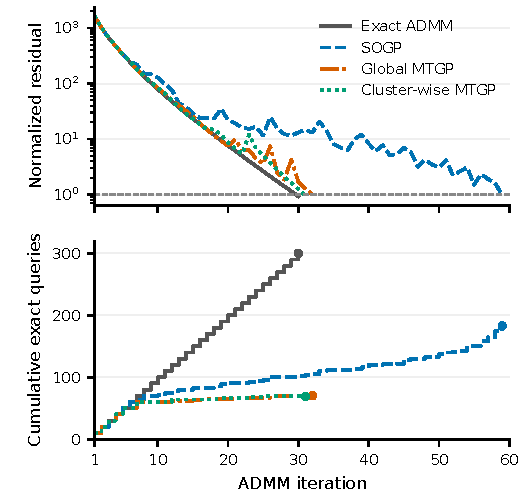
\includegraphics[width=\columnwidth]{figures/verified_diagnostic.pdf}
 \caption{Three overlapping groups, using the settings in Table~\ref{tab:main_results}. Top: maximum of the primal and dual residuals normalized by their respective stopping tolerances; the dashed horizontal line is the stopping boundary. Bottom: cumulative exact agent queries, including the 50 initialization queries. Curves end at each method's termination.}
 \label{fig:verified_diagnostic}
\end{figure}

Figure~\ref{fig:verified_diagnostic} illustrates the tradeoff on the three-group overlapping instance. Global and cluster-wise MTGP terminate after 32 and 31 iterations with 70 and 69 queries, respectively, compared with 30 iterations and 300 queries for exact-update ADMM. SOGP uses 59 iterations and 183 queries. The residual curves report algorithmic progress, while the cumulative counts separately expose the communication cost.

\subsection{Value of Known Group Labels}
For \textbf{RQ2}, the selected cluster-wise and global MTGP runs have similar communication costs. Cluster-wise MTGP saves four, six, and one additional queries for separated $K=2$, overlapping $K=2$, and overlapping $K=3$, respectively; for separated $K=3$, it uses four more queries. Its iteration count is higher in three of the four comparisons. These results do not establish a consistent communication advantage from known labels, nor do they demonstrate that overlap causes negative transfer in global MTGP. The observed gains support joint surrogate modeling across these instances, but do not by themselves verify recovery of the generating groups.

Known labels can reduce the size of each GP system. For dense exact GP factorization, let $m_k=(p+1)\sum_{i\in\mathcal C_k}n_i$ be the number of scalar observations in group $k$, and $m=\sum_km_k$. The global cost is $\mathcal O(m^3)$, whereas the total cluster-wise cost is $\mathcal O(\sum_km_k^3)$. At a fixed, balanced observation count, this gives a factor $K^2$ reduction in the leading factorization work. Actual runtime also depends on query counts, refitting, and implementation, so this is a complexity comparison rather than a measured speedup.

\subsection{Scope of the Evidence}
The study uses six synthetic quadratic instances and one optimization seed. Tuning and evaluation use the same instances, and the methods have different GP parameterizations and fitting budgets. Consequently, the results establish an empirical communication--accuracy tradeoff for these configurations, rather than convergence guarantees, generalization to unseen instances, or a causal attribution to task sharing alone. Repeated instances, a common-configuration or held-out tuning comparison, and matched-budget ablations would strengthen those broader claims.


\section{Conclusion}
\label{sec:conclusion}
We developed a derivative-aware MTGP surrogate for Moreau-envelope gradients to reduce exact agent queries in sharing ADMM. On six synthetic quadratic instances, the selected global MTGP configurations reduce exact exchanges by $76.25$--$80.77\%$, with terminal objective discrepancy below $0.01\%$ from the exact-update ADMM baseline and a modest increase in iterations. Known group labels yield small, mixed communication benefits and permit smaller GP factorizations. These findings are empirical and depend on instance-specific tuning. Future work will investigate convergence conditions for the surrogate updates, repeated-instance evaluation, and adaptive grouping from query data.

\bibliographystyle{ieeetr}
\bibliography{refs}
\end{document}
